\documentclass[../../main]{subfiles}

\renewcommand\thesection{\arabic{section}}


\begin{document}

\section{Design} \label{sec:}

\begin{figure}
    \centering
    \includegraphics [
        max width = \IGXMaxWidth,
        max height = \IGXMaxHeight,
        \IGXDefaultOptionalArgs,
    ] {tikzpics/endCoreBlockPanels.pdf}
    \captionof{figure} {}
    \label{fig:}
\end{figure}

\pagebreak

\subsection{C Mode}

\begin{figure}
    \centering
    \includegraphics [
        max width = \IGXMaxWidth,
        max height = \IGXMaxHeight,
        \IGXDefaultOptionalArgs,
    ] {tikzpics/endCADExhaustCMODE.pdf}
    \captionof{figure} {Exhaust core block in \texttt{CMODE}.}
    \label{fig:}
\end{figure}

\subsection{H Mode}

\begin{figure}
    \centering
    \includegraphics [
        max width = \IGXMaxWidth,
        max height = \IGXMaxHeight,
        \IGXDefaultOptionalArgs,
    ] {tikzpics/endCADExhaustHMODE.pdf}
    \captionof{figure} {Exhaust core block in \texttt{HMODE}.}
    \label{fig:}
\end{figure}

\subsection{E Mode}

\begin{figure}
    \centering
    \includegraphics [
        max width = \IGXMaxWidth,
        max height = \IGXMaxHeight,
        \IGXDefaultOptionalArgs,
    ] {tikzpics/endCADExhaustEMODE.pdf}
    \captionof{figure} {Exhaust core block in \texttt{EMODE}.}
    \label{fig:}
\end{figure}


% \begin{figure}
%     \centering
% \end{figure}
%
% \begin{figure}
%     \centering
%     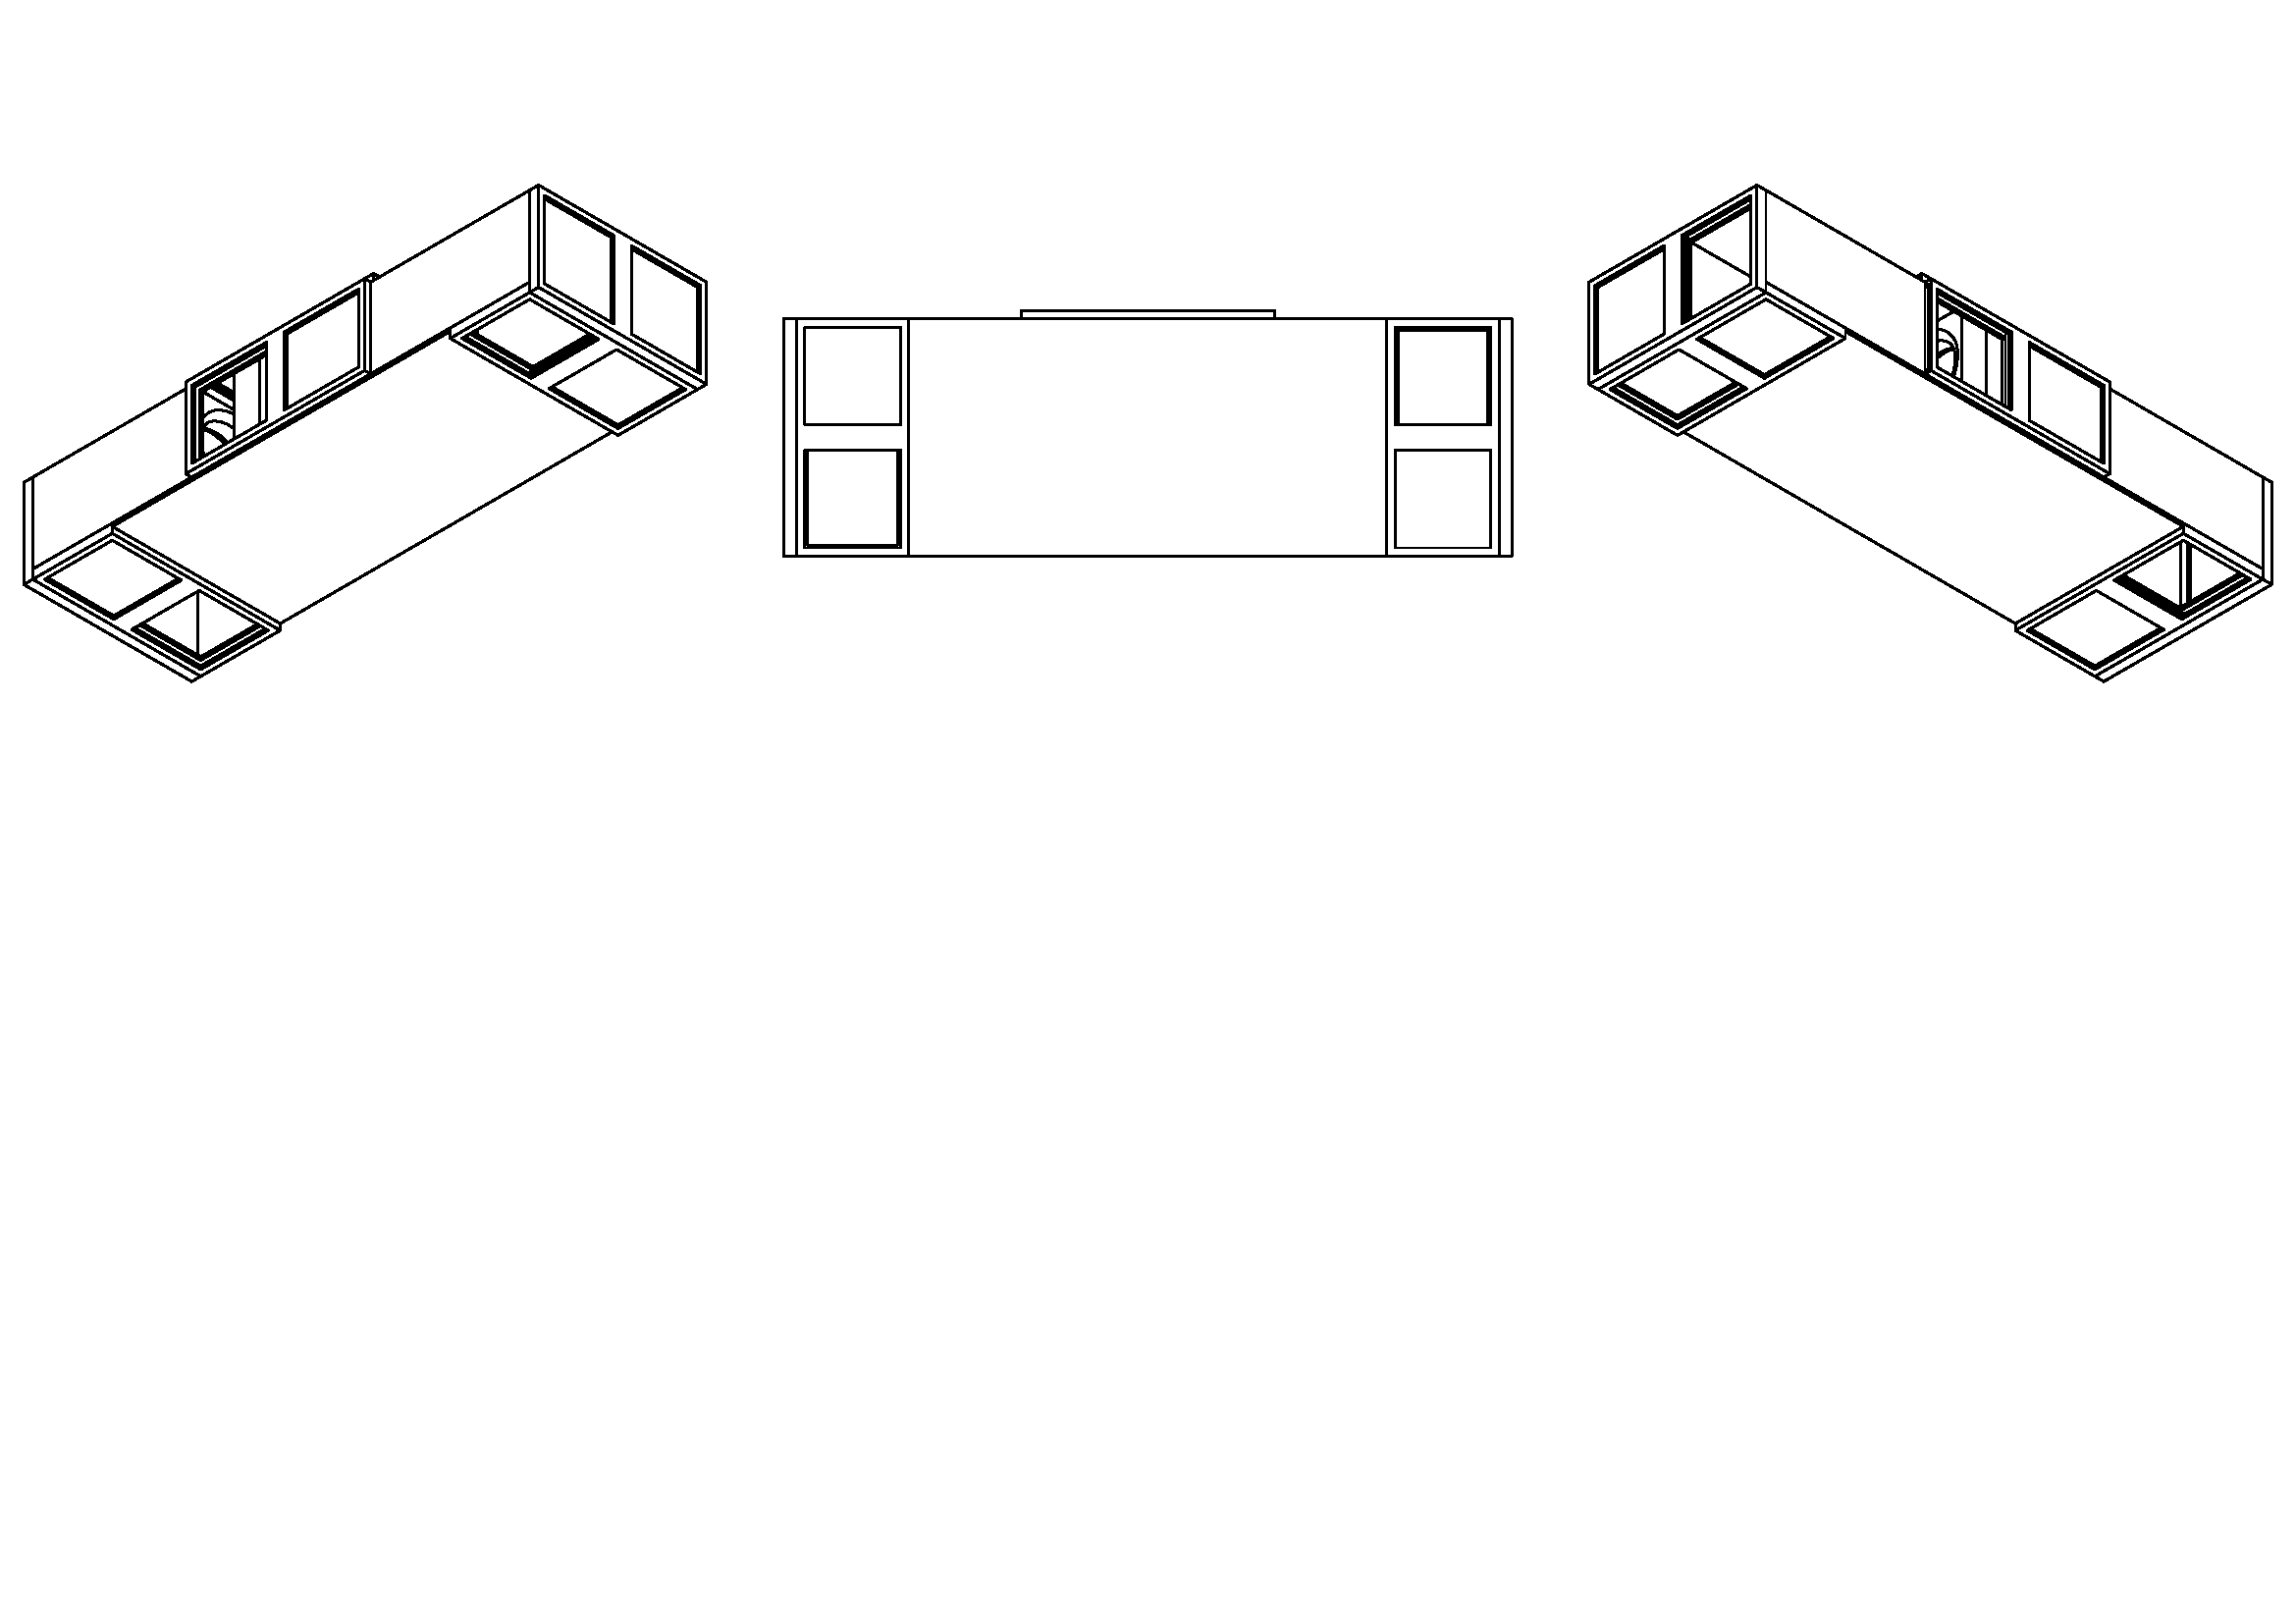
\includegraphics [
%         max width = \IGXMaxWidth,
%         max height = \IGXMaxHeight,
%         \IGXDefaultOptionalArgs,
%         trim = {0 16.25cm 0 3.15cm},
%         clip,
%     ] {pics/cmode_bot.pdf}
%     \captionof{figure} {}
%     \label{fig:}
% \end{figure}
%


\end{document}
